\documentclass{beamer}

\usepackage[utf8]{inputenc}
\usepackage[T1]{fontenc}
\usepackage{textpos}
\usepackage{tikz}

\usetheme{Madrid}
\usecolortheme{beaver}

% Custom changes:
\setbeamertemplate{footline}[frame number]{}
\definecolor{university_tuebingen}{RGB}{165,30,55}
\setbeamercolor{frametitle}{fg=university_tuebingen, bg=white}
\setbeamercolor{title}{fg=university_tuebingen}

\addtobeamertemplate{frametitle}{}{
\begin{tikzpicture}[remember picture, overlay]
\node[anchor=north east,yshift=0cm] at (current page.north east)
{
\includegraphics[width=3cm]{../common/logo_uni_tuebingen2.png}};
\end{tikzpicture}}



\author{Prof. Dr. Christiane Zarfl, Dipl.-Inf. Willi Kappler}
%\date{\today}
\date{}
%\institute{Universität Tübingen}
\institute{}


\title{{
\beamertemplatenavigationsymbolsempty % suppress navigation on this (= first) slide
\begin{frame}[plain] % plain means: no header and footer on this (= first) slide
    \begin{textblock*}{0cm}(0.5cm, -0.7cm)
        
\includegraphics[width=11.0cm]{../common/logo_uni_tuebingen.png}
    \end{textblock*}
    \titlepage
    \begin{textblock*}{0cm}(0.1cm, -2.5cm)
        \textcolor{university_tuebingen}{\rule{11.8cm}{0.2cm}}
    \end{textblock*}
\end{frame}
}
\\{\scriptsize 1. Grundlagen}}

\setcounter{mexercise}{1}

\begin{document}
    {
\beamertemplatenavigationsymbolsempty % suppress navigation on this (= first) slide
\begin{frame}[plain] % plain means: no header and footer on this (= first) slide
    \begin{textblock*}{0cm}(0.5cm, -0.7cm)
        
\includegraphics[width=11.0cm]{../common/logo_uni_tuebingen.png}
    \end{textblock*}
    \titlepage
    \begin{textblock*}{0cm}(0.1cm, -2.5cm)
        \textcolor{university_tuebingen}{\rule{11.8cm}{0.2cm}}
    \end{textblock*}
\end{frame}
}


    \section{Einleitung}
    \begin{frame}
      \frametitle{Inhaltsverzeichnis}
      \tableofcontents[currentsection, hideallsubsections]
    \end{frame}

    \subsection{Warum Matlab ?}
    \begin{frame}
      \frametitle{Matlab - Warum ?}
      \begin{textblock*}{0cm}(5.0cm, -1.0cm)
        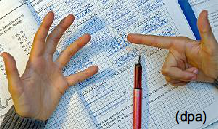
\includegraphics[width=3.0cm]{rechnen1.png}
      \end{textblock*}
      \begin{textblock*}{0cm}(9.0cm, 0.0cm)
        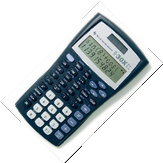
\includegraphics[width=2.0cm]{rechnen2.png}
      \end{textblock*}

      \begin{itemize}
        \itemsep0.4cm
        \item Einfache Rechnungen
        \item Datenaufbereitung \& -speicherung
        \item Visualisierung von Daten \& Simulationsergebnissen
        \item einfaches Lösen von (linearen) Gleichungssystemen, Differentialgleichungen (DGL), DGL-Systemen...
        \item Wiederverwendung von häufig gebrauchten Berechnungen (Programmierung)
        \item Datenanalyse (z.B. Regression) \& Statistik
        \item Komplexe Modellierung von Umweltsystemen
      \end{itemize}
    \end{frame}

    \subsection{Visualisierung}
    \begin{frame}
      \frametitle{Matlab - Warum ?}
      \vspace{-0.8cm}
      \begin{figure}
        Visualisierung von Daten \& Simulationsergebnissen \par \vspace{0.4cm}
        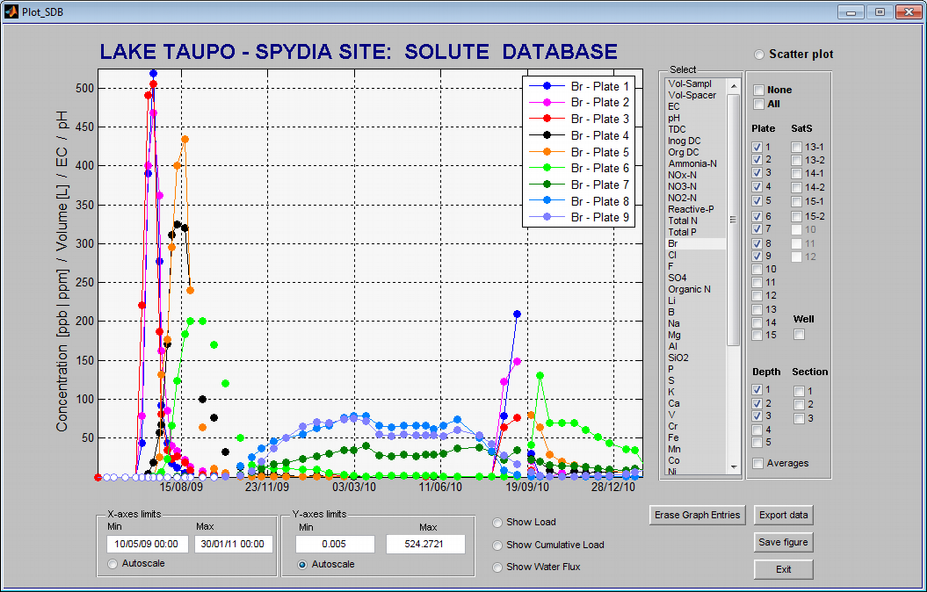
\includegraphics[width=10.0cm]{visualisierung1.png}
      \end{figure}
    \end{frame}

    \subsection{Datenalalyse}
    \begin{frame}
      \frametitle{Matlab - Warum ?}

      \vspace{-0.8cm}

      \begin{figure}
        Datenanalyse \& Statistik \par \vspace{0.4cm}
        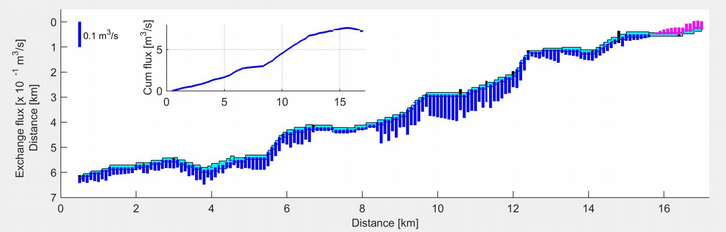
\includegraphics[width=10.0cm]{visualisierung2.png}
      \end{figure}

      \vspace{-0.5cm}

      \begin{figure}
        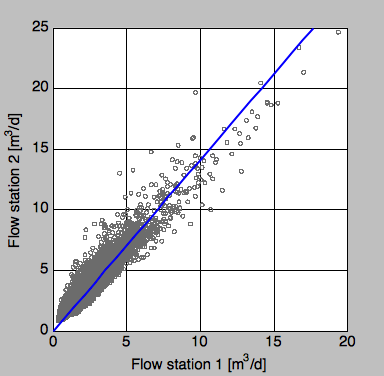
\includegraphics[width=3.0cm]{visualisierung3.png}
        \hspace{0.5cm}
        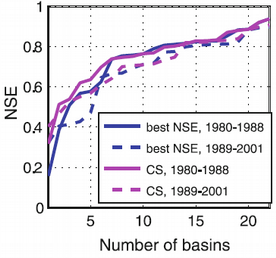
\includegraphics[width=3.0cm]{visualisierung5.png}
        \hspace{0.5cm}
        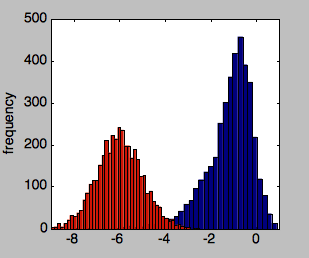
\includegraphics[width=3.0cm]{visualisierung4.png}
      \end{figure}
    \end{frame}

    \subsection{Modellierung}
    \begin{frame}
      \frametitle{Matlab - Warum ?}
      \vspace{-0.8cm}
      \begin{figure}
        Modellierung von Umwelstsystemen \par \vspace{0.4cm}
        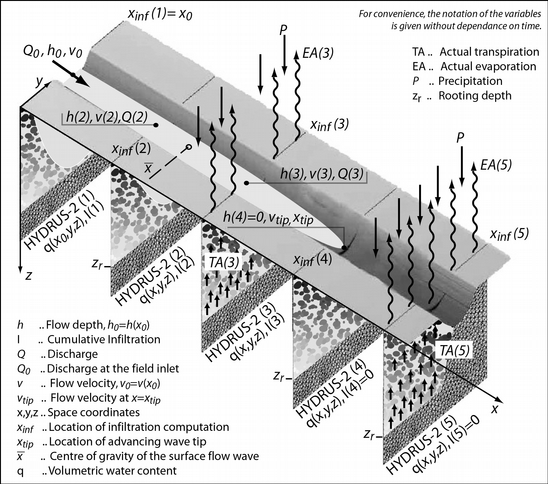
\includegraphics[width=7.5cm]{modellierung1.png}
      \end{figure}
    \end{frame}

    \subsection{Organisatorisches}
    \begin{frame}
        \frametitle{Organisatorisches}

        \vspace{-1.0cm}

        \begin{itemize}
          \item Hardware:

          \begin{itemize}
            \itemsep0.3cm
            \item BYOD (eigenes Gerät mitbringen)
            \item Geo-Notebooks (Raum S245)
            \item CIP Pool Rechner (Raum S310)
          \end{itemize}

          \item Software:

          \begin{itemize}
            \itemsep0.3cm
            \item Auf Institutshardware bereits vorinstalliert
            \item ZDV: Matlab \href{https://services.zdv.uni-tuebingen.de/CampusSoftware/}{\beamergotobutton{hier}} herunterladen
            \item GNU Octave \href{https://www.gnu.org/software/octave/}{\beamergotobutton{Webseite}} (Open Source, aber nicht 100\% compatibel)
          \end{itemize}

          \item \alert{Auf Institutshardware bitte zuerst ein eigenes Verzeichnis anlegen!}

        \end{itemize}
    \end{frame}

    \subsection{Was ist Matlab}
    \begin{frame}
        \frametitle{Was ist Matlab}

        \begin{itemize}
          \item ``\emph{Matlab} ist eine kommerzielle Software des Unternehmens \emph{The MathWorks, Inc.} zur Lösung mathematischer Probleme
          und zur grafischen Darstellung der Ergebnisse.'' (Quelle: \href{https://de.wikipedia.org/wiki/Matlab}{\beamergotobutton{Wikipedia}}).
          \item Matlab leitet sich ab von \textbf{MAT}rix \textbf{LAB}oratory.
          \item Wir benutzen Matlab als (nummerische) Programmiersprache.
          \item Wie ein Taschenrechner oder Excel arbeitet Matlab nummerisch (mit Zahlenwerten, also nicht symbolisch wie
          ein \href{https://de.wikipedia.org/wiki/Computeralgebrasystem}{\beamergotobutton{CAS}}).
          \item Anders als bei einem Taschenrechner können Zahlenwerten Variablennamen zugewiesen werden.
          \item Im Programm werden die Variablennamen als Platzhalter für die Werte verwendet.
        \end{itemize}
    \end{frame}

    \subsection{Ausblick}
    \begin{frame}
        \frametitle{Nach dieser ersten Kurseinheit...}

        \begin{itemize}
          \itemsep0.3cm
          \item kennen Sie den Aufbau der Oberfläche der Software Matlab.
          \item benutzen Sie die Matlab-Hilfe, um für Sie nützliche Funktionen und Informationen selbstständig zu finden.
          \item führen Sie einfache Rechnungen mit Matlab durch.
          \item können Sie Variablen in Matlab definieren und verwenden.
          \item kennen Sie die Vorteile der Verwendung von Vektoren und können diese in Matlab definieren und für Rechnungen verwenden.
        \end{itemize}
    \end{frame}

    \subsection{GUI}
    \begin{frame}
      \frametitle{Die Matlab GUI}

      \vspace{-0.8cm}

      \begin{figure}
        \begin{tikzpicture}
          \node[anchor=south west,inner sep=0] (image) at (0,0) {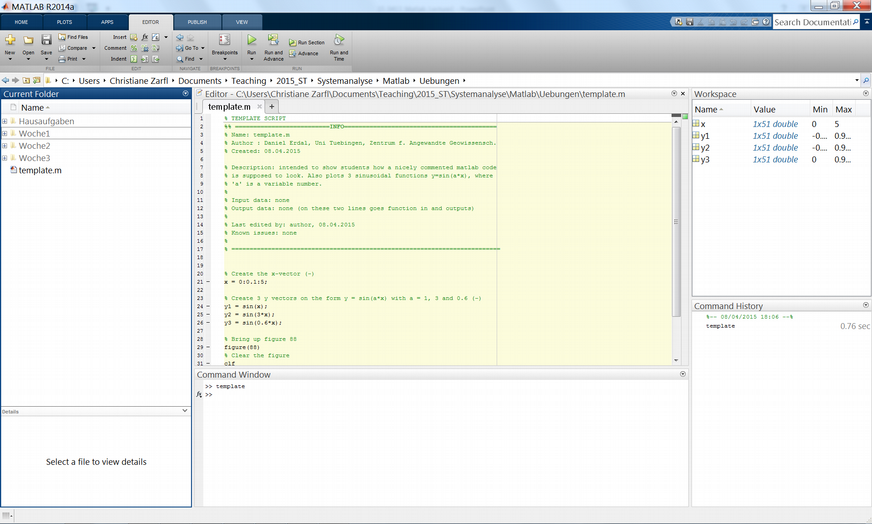
\includegraphics[width=10.0cm]{matlab_gui1.png}};
          \begin{scope}[x={(image.south east)},y={(image.north west)}]
            \node (a) at (0.5, 1.05) {gegenwärtiges Verzeichnis};
            \node[align=left] (b) at (0.1, 0.4) {Dateien im \\gegenwärtigen \\Verzeichnis};
            \node[align=left] (c) at (0.5, 0.5) {Variablen im \\Arbeitsspeicher};
            \node[align=left] (d) at (0.5, 0.15) {Eingabefenster mit \\``Prompt'' (>>)};
            \node[align=left] (e) at (0.85, 0.15) {Eingabe-\\verlauf};
            \draw[line width=0.1cm, ->] (a) -- +(0, -0.2);
            \draw[line width=0.1cm, ->] (b) -- +(0, 0.25);
            \draw[line width=0.1cm, ->] (c) -- +(0.3, 0.15);
            \draw[line width=0.1cm, ->] (e) -- +(0, 0.2);
          \end{scope}
        \end{tikzpicture}
      \end{figure}
    \end{frame}

    \subsection{Hilfe}
    \begin{frame}
      \frametitle{Hilfe in Matlab}
      \begin{itemize}
        \itemsep0.3cm
        \item Niemand kann alle Befehle kennen, deshalb ist die (ausführliche) Hilfe in Matlab so wichtig.
        \item Allgemeines Hilfe-Fenster: \menu{Help > Documentation} (\keys{F1})
        \item Information zu einem Befehl:

        \usebeamercolor{block body example}
        \begin{itemize}
          \itemsep0.3cm
          \item \colorbox{bg}{\texttt{doc <Befehlsname>}} (Info in einem extra Fenster)
          \item \colorbox{bg}{\texttt{help <Befehlsname>}} (Info im Befehlsfenster)
        \end{itemize}

        \item Beispiele: Im Prompt eingeben:

        \begin{itemize}
          \itemsep0.3cm
          \item \colorbox{bg}{\texttt{help sin}}
          \item \colorbox{bg}{\texttt{help exp}}
          \item \colorbox{bg}{\texttt{doc plot}}
        \end{itemize}
      \end{itemize}
    \end{frame}

    \section{Grundlagen}
    \subsection{Einfaches Rechnen}
    \begin{frame}
      \frametitle{Einfaches Rechnen mit Matlab}
      \begin{itemize}
        \itemsep0.3cm
        \usebeamercolor{block body}
        \item Alle Anweisungen werden nach dem Prompt (>>) eingegeben und mit \keys{\return} (Return) bestätigt. Matlab nennt das Ergebnis \colorbox{bg}{\texttt{ans}} (für answer):
        \usebeamercolor{normal text}

        \begin{columns}[t]
          \begin{column}{5cm}
            \usebeamercolor{block body example}
            \colorbox{bg}{\lstinputlisting[language=Matlab]{example1.1.m}}
          \end{column}

          \begin{column}{5cm}
            \usebeamercolor{block body}
            \colorbox{bg}{\lstinputlisting[language=Matlab]{example1.1.txt}}
          \end{column}
        \end{columns}

        \item Addition ($\oplus$), Subtraktion ($\ominus$), Multiplikation ($\otimes$) und Division ($\oslash$) wie im Taschenrechner (Matlab kennt ``Punkt vor Strich-Rechnung'').
        \item Braucht man einen \textbf{Ausdruck öfters}, so kann man ihn als \textbf{Variable} definieren:

        \vspace{0.3cm}

        \begin{columns}[t]
          \begin{column}{5cm}
            \usebeamercolor{block body example}
            \colorbox{bg}{\lstinputlisting[language=Matlab]{example1.2.m}}
          \end{column}

          \begin{column}{5cm}
            \usebeamercolor{block body}
            \colorbox{bg}{\lstinputlisting[language=Matlab]{example1.2.txt}}
          \end{column}
        \end{columns}

        \item Variablen werden im Arbeitsspeicher (Workspace) gespeichert (s. Arbeitsspeicher-Fenster).
      \end{itemize}
    \end{frame}

    \begin{frame}
      \frametitle{Grundlegendes}
      \begin{itemize}
        \item Ein Semikolon (;) am Ende der Eingabezeile unterdrückt die Ausgabe des Ergebnisses.
        \item Matlab \textbf{unterscheidet} zwischen Groß- und Kleinbuchstaben!
        \item Potenzieren wird \textbf{vor} einer \textbf{Multiplikation} oder \textbf{Division} ausgewertet, sonst gilt ``Punkt-vor-Strich''; runde Klammern ``('' und ``)'' um die Reihenfolge der Berechnung zu steuern.
        \item Mehrere Anweisungen in einer Zeile sind zulässig:

        \begin{itemize}
          \item Sind sie durch ein Komma getrennt, so folgt eine Ausgabe.
          \item Werden sie durch ein Semikolon getrennt, so folgt keine Ausgabe:

          \vspace{0.3cm}

          \begin{columns}[t]
            \begin{column}{5cm}
              \usebeamercolor{block body example}
              \colorbox{bg}{\lstinputlisting[language=Matlab]{example1.3.m}}
            \end{column}

            \begin{column}{5cm}
              \usebeamercolor{block body}
              \colorbox{bg}{\lstinputlisting[language=Matlab]{example1.3.txt}}
            \end{column}
          \end{columns}

        \end{itemize}
      \end{itemize}
    \end{frame}

    \subsection{Variablen}
    \begin{frame}
      \frametitle{Regeln für Variablen}
      \begin{itemize}
        \item Regeln bei der Definition von Variablen:
        \item Das erste Zeichen muss ein Buchstabe sein (Keine Zahl!)
        \item Keine Sonderzeichen (außer Unterstrich)
        \item Max. Zeichenlänge (abhängig vom Computer)
        \item \alert{Vorsicht:} Variablennamen identisch mit Funktionen ist erlaubt, hat aber Seiteneffekte!
        \item Variablen haben einen bestimmten \textbf{Typ}, z.B. Ganzzahl, Fließkommazahl, Vector, Matrix, ...
      \end{itemize}
    \end{frame}

    \begin{frame}
      \frametitle{Auflisten und löschen von Variablen}
      \begin{itemize}
        \item \texttt{who:} gibt eine Liste der Variablen im Arbeitsspeicher aus
        \item \texttt{whos:} gibt zusätzliche Information (Typ, Größe, Speicherbedarf)
        \item \texttt{clear <Variable>:} löscht die Variable
        \item \texttt{clear all:} löscht alle Variablen
        \item \texttt{clc:} löscht den Inhalt des Befehlsfensters
      \end{itemize}
    \end{frame}

    \subsection{\mexercise}
    \begin{frame}
      \frametitle{\mexercise}
      \begin{exercise}
          Geben Sie nacheinander folgende Anweisungen ein. Überlegen Sie vorher was wird Matlab ausgeben? \\ \\
          \texttt{u = 2,v = 5;} \keys{\return}\\
          \texttt{(u+6)/4} \keys{\return}\\
          \texttt{y = x+1} \keys{\return}\\
          \texttt{y = 3u} \keys{\return}\\ \\
          Welche der folgenden Variablennamen sind \textbf{nicht} zulässig? \\ \\
          \texttt{anzahl}, \texttt{Summe\_a+b}, \texttt{5\_Tageskarte}, \texttt{dauer\_phase3}, \texttt{sin}
      \end{exercise}
  \end{frame}

  \subsection{Funktionen}
  \begin{frame}
    \frametitle{Einfache Funktionen}
    \begin{itemize}
      \item Es gibt in Matlab bereits ``eingebaute'' Funktionen (viel mehr als im Taschenrechner und Excel).
      \item Z.B. die Wurzelfunktion (square root): \texttt{a = sqrt(2)/2}
      \item Nähere Informationen zur Funktion \texttt{sqrt} erhält man mit \texttt{help sqrt}.
      \item Funktionen können keinen, einen oder mehrere \textbf{Eingabeparameter} haben.
      \item Funktionen können keinen, einen oder mehrere \textbf{Rückgabewerte} haben.
      \item Wie bei Variablen auch haben Funktionen einen bestimmten Typ. D.h. die Ein- und Ausgabewerte \textbf{müssen} vom Typ her passen.
    \end{itemize}
  \end{frame}

  \stepcounter{mexercise}
  \subsection{\mexercise}
  \begin{frame}
    \frametitle{\mexercise}
    \begin{exercise}
        Berechnen Sie den natürlichen Logarithmus von \texttt{1.36} \\ \\
        Berechnen Sie auch den Logarithmus zur Basis \texttt{10} von \texttt{1.36} \\ \\
        (Zusatz: Wie berechnen Sie den Logartihmus zur Basis \texttt{3} von \texttt{1.36}?)
    \end{exercise}
\end{frame}

\stepcounter{mexercise}
\subsection{\mexercise}
\begin{frame}
  \frametitle{\mexercise}
  \begin{exercise}
      Berechnen Sie \texttt{cos($\pi$)} und \texttt{cos($\pi / 2$)} \\ \\
      $\pi$ ist in Matlab bereits eingebaut und wird mit \texttt{pi} bezeichnet \\ \\
      \alert{Vorsicht}: Das Argument der trigonometrischen Funktionen (\texttt{sin, cos, tan, cot}) wird von Matlab immer im \textbf{Bogenmaß} interpretiert \\ \\
      Berechnen Sie den Kosinus von \texttt{180$^{\circ}$} und \texttt{90$^{\circ}$}
  \end{exercise}
\end{frame}

\subsection{Zahlen, Vektoren und Matrizen}
\begin{frame}
  \frametitle{Zahlen, Vektoren und Matrizen in Matlab}
  \begin{itemize}
      \item Eine Gruppierung von mehreren Zahlenwerten nennt man einen \textbf{Vektor}
      \item Eine zweidimensionale Gruppierung von Zahlen nennt man eine \textbf{Matrix}
      \item \textbf{Es folgt:} Eine Zahl ist sowohl ein spezieller Vektor (der Länge \texttt{1}), als auch eine spezielle Matrix der Dimension \texttt{1$\times$1}.
      \item \textbf{Ein Vektor der Länge n} ist eine spezielle Matrix der Dimension \texttt{n$\times$1} (Spaltenvektor) oder \texttt{1$\times$n} (Zeilenvektor)
      \item Matlab (\textbf{MAT}rix \textbf{LAB}oratory) kennt intern nur Matrizen!
      \item Die Berechnung der Wurzel in Matlab von vorhin: \\
      \texttt{a = sqrt(2)/2} \\
      Hier ist \texttt{a} eine \texttt{1$\times$1} Matrix (Selbst die Konstante \texttt{2} wird als eine konstante \texttt{1$\times$1} Matrix interpretiert)
  \end{itemize}
\end{frame}






\end{document}
